\RequirePackage{plautopatch}
\documentclass[14pt,aspectratio=169,xcolor=dvipsnames,table,onlytextwidth,dvipdfmx]{beamer}
\usepackage[utf8]{inputenc}
\usepackage{bxdpx-beamer} % dvipdfmxなので必要

\usetheme{Boadilla}
%Beamerフォント設定
\usefonttheme{professionalfonts}
\usepackage[T1]{fontenc}
\usepackage[deluxe,uplatex]{otf} % 日本語多ウェイト化
\usepackage{mlmodern}  % 太いComputer Modern
% MLmodernのバグを修正: cf. https://tex.stackexchange.com/questions/646333/size-of-integral-symbol-in-section-header-with-mlmodern
\DeclareFontFamily{OMX}{mlmex}{}
\DeclareFontShape{OMX}{mlmex}{m}{n}{%
   <->mlmex10%
   }{}
\usepackage{newtxtext} % 数式以外をTXフォントで上書き
% \usepackage[noalphabet,unicode]{pxchfon}
% \setminchofont{KozMinPro-Regular.otf}% 游明朝Regular
% \setboldminchofont{KozMinPro-Bold.otf}% 游明朝Demibold
% \setgothicfont[0]{BIZ-UDGothicR.ttc}% BIZ UDゴシックR
% \setboldgothicfont[0]{BIZ-UDGothicB.ttc}% BIZ UDゴシックB
\renewcommand{\familydefault}{\sfdefault}  % 英文をサンセリフ体に
\renewcommand{\kanjifamilydefault}{\gtdefault}  % 日本語をゴシック体に
\usefonttheme{structurebold} % タイトル部を太字
\setbeamerfont{alerted text}{series=\bfseries} % Alertを太字
\setbeamerfont{section in toc}{series=\mdseries} % 目次は太字にしない
\setbeamerfont{frametitle}{size=\Large} % フレームタイトル文字サイズ
\setbeamerfont{title}{size=\LARGE} % タイトル文字サイズ
\setbeamerfont{date}{size=\small}  % 日付文字サイズ
\usepackage{bxcoloremoji}

% Babel (日本語の場合のみ・英語の場合は不要)
\uselanguage{japanese}
\languagepath{japanese}
\deftranslation[to=japanese]{Theorem}{定理}
\deftranslation[to=japanese]{Lemma}{補題}
\deftranslation[to=japanese]{Example}{例}
\deftranslation[to=japanese]{Examples}{例}
\deftranslation[to=japanese]{Definition}{定義}
\deftranslation[to=japanese]{Definitions}{定義}
\deftranslation[to=japanese]{Problem}{問題}
\deftranslation[to=japanese]{Solution}{解}
\deftranslation[to=japanese]{Fact}{事実}
\deftranslation[to=japanese]{Proof}{証明}
\def\proofname{証明}
\setbeamertemplate{theorems}[normal font] %日本語の場合,定理内を斜体にしない

%Beamer色設定
\definecolor{UniBlue}{RGB}{0,150,200}
\definecolor{UniGreen}{RGB}{3,175,122}
\definecolor{UniPink}{RGB}{255,128,255}
\definecolor{AlertOrange}{RGB}{255,76,0}
\definecolor{AlmostBlack}{RGB}{38,38,38}
\setbeamercolor{normal text}{fg=AlmostBlack}  % 本文カラー
\setbeamercolor{structure}{fg=UniBlue} % 見出しカラー
\setbeamercolor{block title}{fg=UniBlue!50!black} % ブロック部分タイトルカラー
\setbeamercolor{alerted text}{fg=AlertOrange} % \alert 文字カラー
\setbeamercolor{bibliography entry author}{fg=AlmostBlack} % Bib 文字カラー
\setbeamercolor{bibliography entry note}{fg=AlmostBlack} % Bib 文字カラー
\mode<beamer>{
    \definecolor{BackGroundGray}{RGB}{254,254,254}
    \setbeamercolor{background canvas}{bg=BackGroundGray} % スライドモードのみ背景をわずかにグレーにする
}

%フラットデザイン化
\setbeamertemplate{blocks}[rounded] % Blockの影を消す
\useinnertheme{circles} % 箇条書きをシンプルに
\setbeamertemplate{navigation symbols}{} % ナビゲーションシンボルを消す
\setbeamertemplate{footline}[frame number] % フッターはスライド番号のみ

%タイトルページ
\setbeamertemplate{title page}{%
    \vspace{2.5em}
    {\usebeamerfont{title} \usebeamercolor[fg]{title} \inserttitle \par}
    {\usebeamerfont{subtitle}\usebeamercolor[fg]{subtitle}\insertsubtitle \par}

    \vspace{1.5em}
    \begin{columns}[]
        \begin{column}{.35\linewidth}
        \usebeamerfont{titlegraphic}\inserttitlegraphic\par
        \end{column}
        \begin{column}{.6\linewidth}\setlength\topsep{0pt}
            \begin{flushright}
        \usebeamerfont{author}\insertauthor\par
        \usebeamerfont{institute}\insertinstitute \par
        \vspace{3em}
        \usebeamerfont{date}\insertdate\par
            \end{flushright}
        \end{column}
    \end{columns}
}

%biblatex
% \usepackage[style=ext-authoryear,citestyle=authoryear,natbib=true,giveninits=true,maxbibnames=99,maxcitenames=10,url=false,isbn=false,doi=false,articlein=false]{biblatex}
% \DeclareNameAlias{author}{first-last}
% \addbibresource{shrunk.bib}
% \newcommand{\mkbibbracketscol}[1]{\textcolor{UniBlue}{\scriptsize \mkbibbrackets{#1}}}
% \DeclareCiteCommand{\cite}[\mkbibbracketscol]
%   {\usebibmacro{prenote}}
%   {\usebibmacro{citeindex}%
%    \usebibmacro{cite}}
%   {\multicitedelim}
%   {\usebibmacro{postnote}}
% % \renewcommand{\cite}[1]{\textcolor{UniBlue}{\scriptsize\citep{#1}}}
% \renewcommand*{\finalnamedelim}{\addcomma\addspace} % remove "and" before the last author
% \DeclareDelimFormat{nameyeardelim}{\addspace}
% \setbeamertemplate{bibliography item}{}

% Algorithm系
\usepackage{algorithm}
\usepackage[noend]{algorithmic}
\algsetup{linenosize=\color{fg!50}\footnotesize}
\renewcommand\algorithmicdo{:}
\renewcommand\algorithmicthen{:}
\renewcommand\algorithmicrequire{\textbf{Input:}}
\renewcommand\algorithmicensure{\textbf{Output:}}

% TikZ
\usepackage{tikz}
\usetikzlibrary{positioning,shapes,arrows,quotes,shapes.callouts,calc,graphs,graphs.standard,fit,backgrounds,perspective}
\tikzset{point/.style={circle, fill=AlertOrange, inner sep=1pt, text width=1pt}}
\tikzset{bpoint/.style={circle, fill=black, inner sep=1pt, text width=1pt}}
\tikzset{alt/.code args={<#1>#2#3}{\alt<#1>{\pgfkeysalso{#2}}{\pgfkeysalso{#3}}}}
\tikzset{>=latex}
\tikzset{mynodes/.style={circle,white,fill=UniBlue!90,text width=.8em,inner sep=0pt,text centered,font=\footnotesize}}
\tikzset{myedges/.style={thick}}
\tikzset{mypath/.style={ultra thick, draw=AlertOrange}}
\tikzset{mypath2/.style={ultra thick, dashed, draw=UniGreen}}
\tikzset{mysubset/.style={draw,UniBlue,dotted,thick,fill=UniBlue!10}}
\tikzset{graphs/mygraph/.style={nodes={mynodes}, edges={myedges}, empty nodes}}
%% graph macros
\tikzgraphsset{declare={mybipartite}{%
subgraph I_nm [V={1,2,3,4,5,6}, W={a,b,c,d,e,f}];
1 -- {a,b};
2 -- {b,c,d,e};
3 -- {d,f};
4 -- {e,f};
{5,6} -- f;
}}
\tikzgraphsset{declare={mybipartitedi}{%
subgraph I_nm [V={1,2,3,4,5,6}, W={a,b,c,d,e,f}];
1 -> {a,b};
2 -> {b,c,d,e};
3 -> {d,f};
4 -> {e,f};
{5,6} -> f;
}}
\tikzgraphsset{declare={mybipartite2}{%
subgraph I_nm [V={1,2,3}, W={a,b,c}];
1 -- {a,b}; 2 -- {a,b,c}; 3 -- {a,c};
}} 

% Appendix
\usepackage{appendixnumberbeamer}

% macros
\newcommand{\R}{\mathbb{R}}
\newcommand{\Z}{\mathbb{Z}}
\newcommand{\be}{\mathbf{e}}
\newcommand{\ones}{\mathbf{1}}
% \newcommand{\bp}{\mathbf{p}}
\newcommand{\eps}{\varepsilon}
\newcommand{\defiff}{\overset{\text{def}}{\iff}}
\DeclareMathOperator{\poly}{poly}

\usepackage{mathtools}
\DeclarePairedDelimiter{\abs}{\lvert}{\rvert}
\DeclarePairedDelimiter{\norm}{\lVert}{\rVert}
\DeclarePairedDelimiter{\inprod}{\langle}{\rangle}
\usepackage[no-test-for-array]{nicematrix}
\usepackage{diagbox}

\newcommand{\highlightcap}[3][red]{\tikz[baseline=(x.base)]{\node[rectangle,rounded corners,fill=#1!10](x){#2} node[below=0pt of x, color=#1]{#3};}}
\newcommand{\highlight}[2][red]{\tikz[baseline=(x.base)]{\node[rectangle,rounded corners,fill=#1!10](x){#2};}}
\newcommand{\mycite}[2][\footnotesize]{\textcolor{UniBlue}{#1 [#2]}}

%section
% \AtBeginSection[]{
%     \frame[c]{
%         \centering
%         \begin{tikzpicture}
%             \node[white, circle, fill=UniBlue, text centered, text width=.3\linewidth](bullet) {
%                 {\Huge \bf \insertsectionnumber} \\[4em]
%     };
%     \node[text width=.65\linewidth, right=1em of bullet]{%
%         \usebeamerfont{title}\usebeamercolor[fg]{title}\insertsection\par %
%     };
%         \end{tikzpicture}
%     } %目次スライド
% }

%grid
% \usepackage[colorgrid,gridunit=pt,texcoord]{eso-pic}
\newcommand{\postit}[1]{\tikz[overlay, remember picture]{\node[draw,anchor=north east, align=center, rectangle, fill=yellow!10,xshift=-1pt,yshift=-1pt] at (current page.north east) {#1};}}

\usepackage{tcolorbox}
\newtcolorbox{primal}{colback=red!10!white, colframe=red, title=主問題 (P), left=2pt,right=2pt,top=0pt,bottom=0pt}
\newtcolorbox{dual}{colback=blue!10!white, colframe=blue, title=双対問題 (D), left=2pt,right=2pt,top=0pt,bottom=0pt}

% visible on
\usetikzlibrary{overlay-beamer-styles}

\title{計算数理基礎(多面体的組合せ論)}
\author{担当: \textbf{相馬 輔}}

\begin{document}
\maketitle

\begin{frame}<1>[label=outline]{目次}
\begin{tikzpicture}
    \tikzstyle{block} = [rectangle, text width=\textwidth, rounded corners, minimum height=4em]
    \tikzstyle{line} = [draw, -latex]

    \node[block,alt={<1,3->{fill=cyan!10}{fill=red!10}}] (combopt) {
        \begin{columns}
            \begin{column}{0.40\linewidth}
        \textbf{1. 組合せ最適化とは}
            \end{column}
            \begin{column}{0.5\linewidth}
                \small
                \structure{・} 組合せ最適化とは?\\
                \structure{・} 組合せ最適化問題を「解く」とは?\\
                \structure{・} 多項式時間とは?
            \end{column}
        \end{columns}
    };
    \node[block,alt={<1-2,4->{fill=cyan!10}{fill=red!10}}, below=.5em of combopt] (LP) {
        \begin{columns}
            \begin{column}{0.4\linewidth}
        \textbf{2. 線形計画の復習}
            \end{column}
            \begin{column}{0.5\linewidth}
                \small
                \structure{・} 主問題・双対問題 \\
                \structure{・} 相補性条件 \\
                \structure{・} 多面体
            \end{column}
        \end{columns}
    };
    \node[block,alt={<1-3,5->{fill=cyan!10}{fill=red!10}}, below=.5em of LP] (TU) {
        \begin{columns}
            \begin{column}{0.5\linewidth}
        \textbf{3. 整数多面体,完全単模行列}
            \end{column}
            \begin{column}{0.5\linewidth}
                \small
                \structure{・} 完全単模行列 \\
                \structure{・} 整数多面体 \\
                \structure{・} 整数多面体とLPの整数性 \\
            \end{column}
        \end{columns}
    };
\end{tikzpicture}%
\end{frame}

%%%%%%%%%%%%%%%%%%%%%%%%%%%%%%%%%%%%%%%%%%%%%
\section{組合せ最適化とは}
\againframe<2|handout:0>{outline}
%%%%%%%%%%%%%%%%%%%%%%%%%%%%%%%%%%%%%%%%%%%%%
\begin{frame}
    \frametitle{組合せ最適化とは}
    \alert{離散的}な対象の中から最も良いものを\alert{効率的}に求める方法論

    \vfill
    \begin{columns}[]
        \begin{column}{.3\textwidth}
            \centering
            
\includegraphics[width=\textwidth]{figs/network.jpg}
            ネットワーク
        \end{column}
        \begin{column}{.3\textwidth}
            \centering
        \begin{tikzpicture}[>=latex,scale=.8]
        \foreach \i in {1,2,3} {
            \node[inner sep=0pt](v\i) at ($(0, -\i*2)$) {\coloremojiucs[scale=2]{:factory:}};
            \node[inner sep=0pt](w\i) at ($(4, -\i*2)$) {\coloremojiucs[scale=2]{:convenience_store:}};
        }
        \graph{
            {(v1), (v2), (v3)} --[complete bipartite] {(w1), (w2), (w3)}
        };
        \end{tikzpicture}
            マッチング
        \end{column}
        \begin{column}{.3\textwidth}
            \centering
            % \includegraphics[width=\textwidth]{active.pdf}
            \tikzset{block/.style={draw, thick, rectangle}}
            \begin{tikzpicture}[>=latex]
                \node[block](x1) at (0,2)  {$X_1$};
                \node[block](x2) at (0,1)  {$X_2$};
                \node[]          at (0,0)  {$\vdots$};
                \node[block](xn) at (0,-1) {$X_n$};
                \node[block](y)  at (3,0)  {$Y$};
                \begin{scope}[every path/.style={->,very thick,gray}]
                \draw (x1.east) to [bend left ] (y.west);
                \draw (x2.east) -- (y.west);
                \draw (xn.east) to [bend right] (y.west);
                \end{scope}
            \end{tikzpicture}
            機械学習・統計
        \end{column}
    \end{columns}
\end{frame}

\begin{frame}[t]
    \frametitle{例: 割当問題}
    \begin{columns}[T]
    \begin{column}{.5\textwidth}
        \begin{block}{割当問題}
            \structure{入力} コスト$c_{ij} \in \R$ ($1 \leq i, j \leq n$) \\
            \structure{出力} 総コスト最小のマッチング
        \end{block}

        \vspace{3em}
        \small
        \alert{マッチング}...どの頂点にも1本だけ枝が接続しているような枝部分集合
    \end{column}
    \begin{column}{.5\textwidth}
        \centering
        \begin{tikzpicture}[>=latex]
        \foreach \i in {1,2,3} {
            \node[inner sep=0pt](v\i) at ($(0, -\i*2)$) {\coloremojiucs[scale=2]{:factory:}};
            \node[inner sep=0pt](w\i) at ($(4, -\i*2)$) {\coloremojiucs[scale=2]{:convenience_store:}};
        }
        \graph{
            {(v1), (v2), (v3)} --[complete bipartite] {(w1), (w2), (w3)}
        };
        \path (v1)--(w1) node[midway,above,align=center]{\small 輸送コスト $c_{ij}$ \\ \reflectbox{\coloremoji{🚛}}};
        \node[above=1pt of v1] {$i$};
        \node[above=1pt of w1] {$j$};

        \onslide<2->{
            \graph[edges={UniBlue,very thick}]{
                (v1) -- (w1);
                (v2) -- (w3);
                (v3) -- (w2);
            };
        }
    \end{tikzpicture}\\
    \onslide<2->{総コスト$= c_{11} + c_{23} + c_{32}$.}
    \end{column}
    \end{columns}
\end{frame}

\begin{frame}[t]
    \frametitle{例: 巡回セールスマン問題}
    \begin{columns}[T]
    \begin{column}{.55\textwidth}
        \begin{block}{巡回セールスマン問題}
            \structure{入力} 枝コスト$c_{ij} \in \R$ ($1 \leq i, j \leq n$) \\
            \structure{出力} 各頂点を一度だけ通る閉路で総コスト最小のもの
        \end{block}
    \end{column}
    \begin{column}{.40\textwidth}
    \centering
    \begin{tikzpicture}[xscale=1.2,>=latex]
        \begin{scope}[every node/.style={inner sep=0pt}]
            \node(v1) at (18 :2) {\coloremoji[scale=2]{🗼}};
            \node(v2) at (90 :2) {\coloremoji[scale=2]{🏠}};
            \node(v3) at (162:2) {\coloremoji[scale=2]{🏫}};
            \node(v4) at (234:2) {\coloremoji[scale=2]{🏬}};
            \node(v5) at (306:2) {\coloremoji[scale=2]{🏝}};
        \end{scope}
        \node[above=1pt of v2] {$i$};
        \node[right=1pt of v1] {$j$};
        \graph{
            subgraph K_n[V={(v1), (v2), (v3), (v4), (v5)}];
        };
        \path (v1) -- node[midway,sloped,above,align=center]{\small 枝コスト$c_{ij}$ \\ \reflectbox{\coloremoji{🚶‍♀️}}} (v2);
        \onslide<2->{
        \graph[edges={UniBlue,very thick}]{
            (v2) -> (v1);
            (v1) -> (v3);
            (v3) -> (v5);
            (v5) -> (v4);
            (v4) -> (v2);
        };
        }
    \end{tikzpicture}
    \end{column}
    \end{columns}
\end{frame}

\begin{frame}[t,label=maxcoverage]
    \frametitle{例: 最大被覆問題}

    \begin{columns}[T]
    \begin{column}{.55\textwidth}
        \begin{block}{最大被覆問題}
            \structure{入力} $V$: 基地局候補地の集合, $k \in \Z_+$ \\
            \structure{出力} $S \subseteq V$で$|S| \leq k$かつ$S$に設置したときの被覆範囲が最大となるもの
        \end{block}
    \end{column}
    \begin{column}{.40\textwidth}
    \centering
    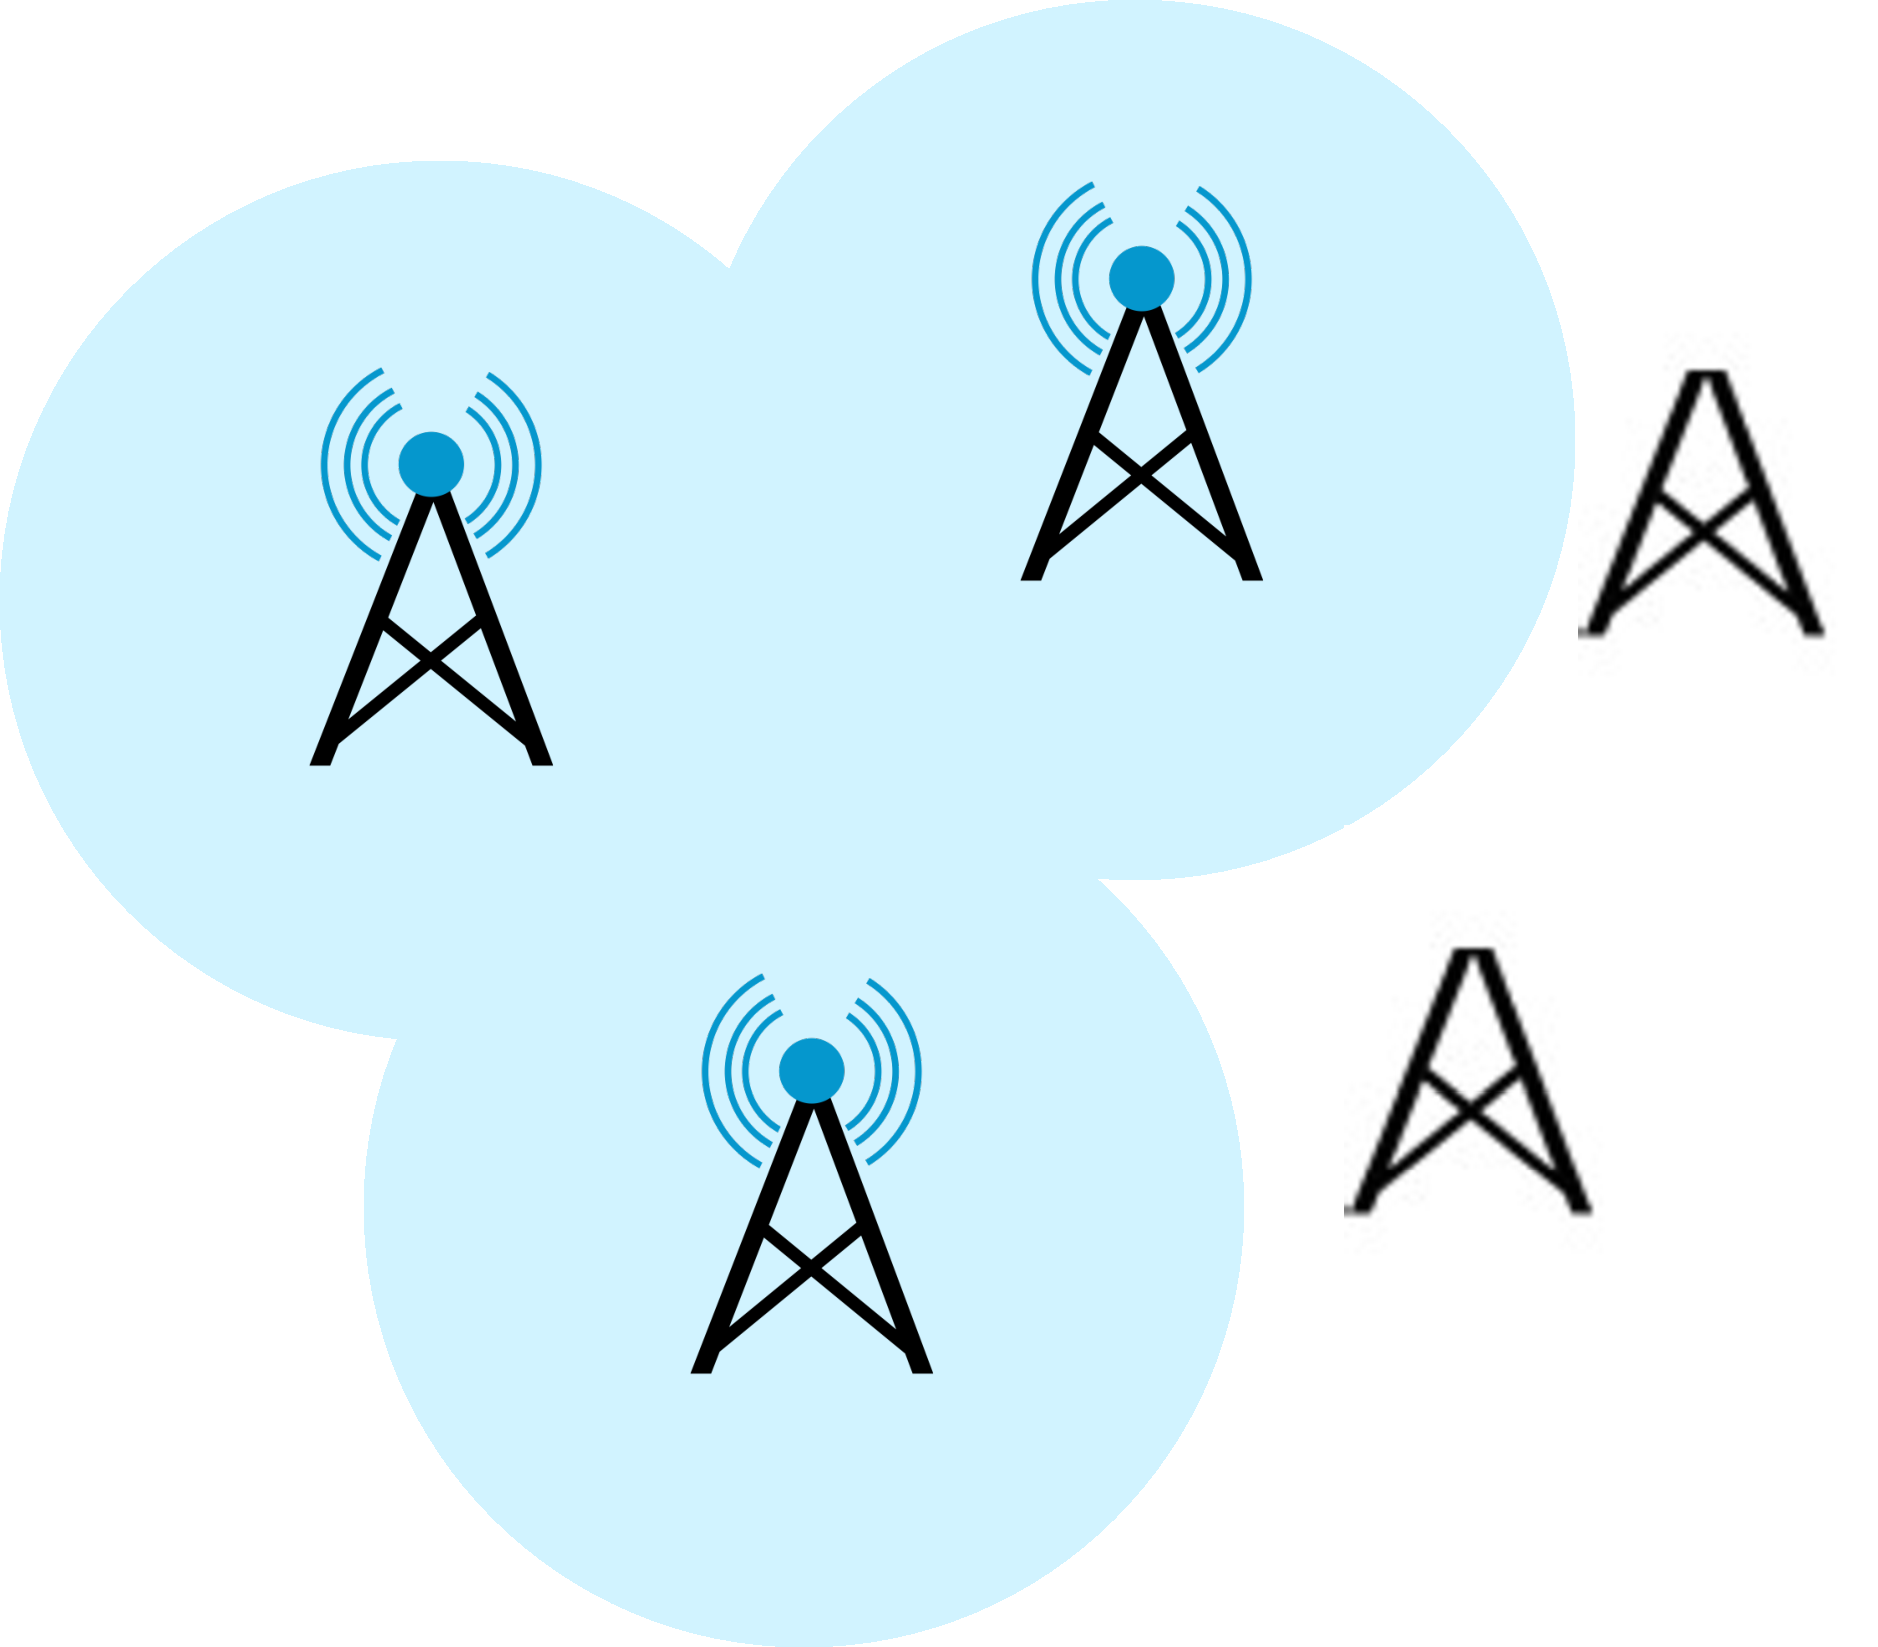
\includegraphics[width=\linewidth]{figs/coverage.pdf}
    \end{column}
    \end{columns}

\end{frame}

\begin{frame}
    \frametitle{愚直な方法: 全探索}
    解をすべて調べて,その中から最適解を選ぶ!
    \pause
    \begin{center}
        \begin{columns}[T]
        \begin{column}{.5\textwidth}
        \centering
        巡回セールスマン問題の場合 \\
        {\scriptsize 1秒間に10京($=10^{17}$)通り調べられるとする.}
        \rowcolors{1}{UniBlue!20}{white}

        \bigskip
        \begin{tabular}{cc}
            頂点数$n$ & 計算時間$\approx n!$ \\ \hline
            10 & $3.6 \times 10^{-11}$秒 \\
            20 & 24秒 \\
            30 & 3168万年
        \end{tabular}
        \end{column}
        \pause
        \begin{column}{.5\textwidth}
            \centering
            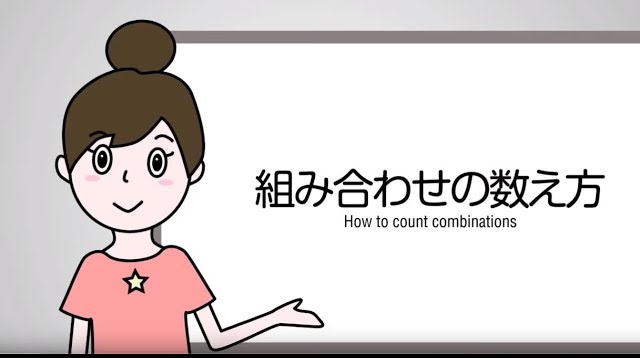
\includegraphics[width=.8\linewidth]{figs/onesan.jpg} \\
            \tiny 引用: 『フカシギの数え方』 おねえさんといっしょ! みんなで数えてみよう!
            \url{https://www.youtube.com/watch?v=Q4gTV4r0zRs}
        \end{column}
        \end{columns}
    \end{center}
    \pause
    現実的ではないので,より\alert{効率的なアルゴリズム}を研究する必要!
    \begin{center}
    \textbf{“効率的”って何だろう?}\coloremoji[scale=1.5]{🤔}
    \end{center}
\end{frame}

\begin{frame}
    \frametitle{アルゴリズムの時間計算量}

    \begin{block}{アルゴリズムの時間計算量}
    入力の大きさ$n$に対して,アルゴリズムが\alert{最大で}何回の\alert{基本演算}\\ 
    (四則演算,大小比較,ビット演算...)を行うかで測る.
    \end{block}
    \pause
    \vfill
    \begin{description}
        \item[多項式時間] 高々$n$の多項式回の基本演算 \\
        \textcolor{UniGreen}{例:} $O(n)$時間,$O(n^2)$時間,$O(n \log n)$時間,$O(n^{10000})$時間
        \item[指数時間] $O(2^n)$回,もしくはそれより大きい回数の基本演算
    \end{description}
    \pause
    \vfill
    \alert{「最大で」}・・・アルゴリズムにとって\textbf{最も苦手}な入力を与えたときにかかる計算量を考える.(最悪時計算量)
\end{frame}

%%%%%%%%%%%%%%%%%%%%%%%%%%%%%%%%%%%%%%%%%%%%%%%%%%%%%
\section{線形計画の復習}
\againframe<3|handout:0>{outline}
%%%%%%%%%%%%%%%%%%%%%%%%%%%%%%%%%%%%%%%%%%%%%%%%%%%%%
\begin{frame}
    \frametitle{線形計画 (LP)}

    LPは以下の標準形で書くことができる:
    \begin{columns}[T]
    \begin{column}{.55\textwidth}
    \begin{block}{}
        \small
        \setlength{\abovedisplayskip}{0pt}
        \begin{alignat*}{2}
            \text{maximize} & \quad  \sum_{j = 1}^n c_j x_j & \\
            \text{subject to} & \quad \sum_{j = 1}^n a_{ij} x_j \leq b_i & \quad (i = 1, \dots, m) \\
            & \quad x_j \geq 0 \quad & (j = 1, \dots, n)
        \end{alignat*}
    \end{block}
    \end{column}
    \begin{column}{.4\textwidth}
        \pause
    \begin{block}{}
        \setlength{\abovedisplayskip}{0pt}
        \begin{alignat*}{2}
            \text{maximize} & \quad  c^\top x \\
            \text{subject to} & \quad A x \leq b  \\
            & \quad x \geq 0 
        \end{alignat*}
    \end{block}
        \footnotesize
        \begin{itemize}
            \item $A$: $m \times n$行列
            \item $b$: $m$次元ベクトル
            \item $c$: $n$次元ベクトル
            \item $x$: $n$次元決定変数
        \end{itemize}
    \end{column}
    \end{columns}
\end{frame}

\begin{frame}
    \frametitle{双対問題・強双対定理}
    \begin{columns}[T]
    \begin{column}{.45\textwidth}
    \begin{primal}
        \setlength{\abovedisplayskip}{0pt}
        \begin{alignat*}{2}
            \text{maximize} & \quad  c^\top x \\
            \text{subject to} & \quad A x \leq b  \\
            & \quad x \geq 0 
        \end{alignat*}
    \end{primal}
    \end{column}
    \begin{column}{.45\textwidth}
    \begin{dual}
        \setlength{\abovedisplayskip}{0pt}
        \begin{alignat*}{2}
            \text{minimize} & \quad  b^\top y \\
            \text{subject to} & \quad A^\top y \geq c  \\
            & \quad y \geq 0 
        \end{alignat*}
    \end{dual}
    \end{column}
    \end{columns}
    
    \vfill
    \pause
    \begin{theorem}[強双対定理]
        主問題(P)と双対問題(D)がともに実行可能ならば,主問題(P)に最適解$x^*$,双対問題(D)に最適解$y^*$が存在して
        $
            c^\top x^* = b^\top y^*
            $
            が成り立つ.
    \end{theorem}
\end{frame}

\begin{frame}
    \frametitle{相補性条件}

    \small
    \begin{columns}[T]
    \begin{column}{.75\textwidth}
    \begin{theorem}[相補性条件]
        主問題(P)の実行可能解$x$と双対問題(D)の実行可能解$y$に対し,$x$と$y$がそれぞれの最適解 \\ 
        $\iff$ 
            $(A^\top y - c)^\top x = 0$
            かつ 
            $(b - Ax)^\top y = 0$  
    \end{theorem}

    \onslide<2->{
    \structure{証明} \\
    実行可能解$(x,y)$に対して,
    \setlength{\abovedisplayskip}{4pt}
    \setlength{\belowdisplayskip}{4pt}
    \[
        c^\top x \leq (A^\top y)^\top x = y^\top (Ax) \leq y^\top b
    \]
    が常に成り立つ(弱双対性).
    }
    \onslide<3->{
    $(x,y)$が最適解ならば,強双対定理から$c^\top x = y^\top b$なので,途中の不等号はすべて等号.よって
    \[
        c^\top x = (A^\top y)^\top x, \quad y^\top (Ax) = y^\top b
    \]
    が成り立つ.移項すると相補性条件が出る.逆も同様. \qed
    }
    \end{column}
    \begin{column}{.2\textwidth}
    \footnotesize
    \begin{primal}
        \setlength{\abovedisplayskip}{0pt}
        \begin{alignat*}{2}
            \text{max} & \quad  c^\top x \\
            \text{s.t.} & \quad A x \leq b  \\
            & \quad x \geq 0 
        \end{alignat*}
    \end{primal}
    \begin{dual}
        \setlength{\abovedisplayskip}{0pt}
        \begin{alignat*}{2}
            \text{min} & \quad  b^\top y \\
            \text{s.t.} & \quad A^\top y \geq c  \\
            & \quad y \geq 0 
        \end{alignat*}
    \end{dual}
    \end{column}
    \end{columns}
\end{frame}

\begin{frame}
    \frametitle{多面体と端点}

    \small
    \begin{columns}[T]
    \begin{column}{.7\textwidth}
    LPの実行可能領域
    \setlength{\abovedisplayskip}{0pt}
    \setlength{\belowdisplayskip}{0pt}
    \begin{align*}
        P = \{ x \in \R^n : Ax \leq b, \, x \geq 0 \} 
        = \{x \in \R^n : 
        \highlightcap[AlertOrange]{$\begin{bmatrix}
            A \\ -I
        \end{bmatrix}$}{$\tilde A$} x \leq 
        \highlightcap[UniBlue]{$\begin{bmatrix}
            b \\ 0
        \end{bmatrix}$}{$\tilde b$}
        \}
    \end{align*}
    は\alert{多面体 (polyhedron)}と呼ばれる凸集合.

    \begin{lemma}
        多面体$P$の端点を$x$とする.このとき,次を満たす大きさ$n$の行部分集合$S$が存在する.
        \begin{itemize}
            \setlength{\itemsep}{0pt}
            \item \highlight[AlertOrange]{$\tilde A$}から$S$に対応する行を抜き出した部分行列$\tilde A_S$は正則
            \item $x$は線形方程式$(\tilde A_S) x = \tilde b_S$の(一意)解.ここで,$\tilde b_S$は$b$から$S$に対応する行を抜き出したベクトル.
        \end{itemize}
    \end{lemma}
    \end{column}
    \begin{column}{.3\textwidth}
        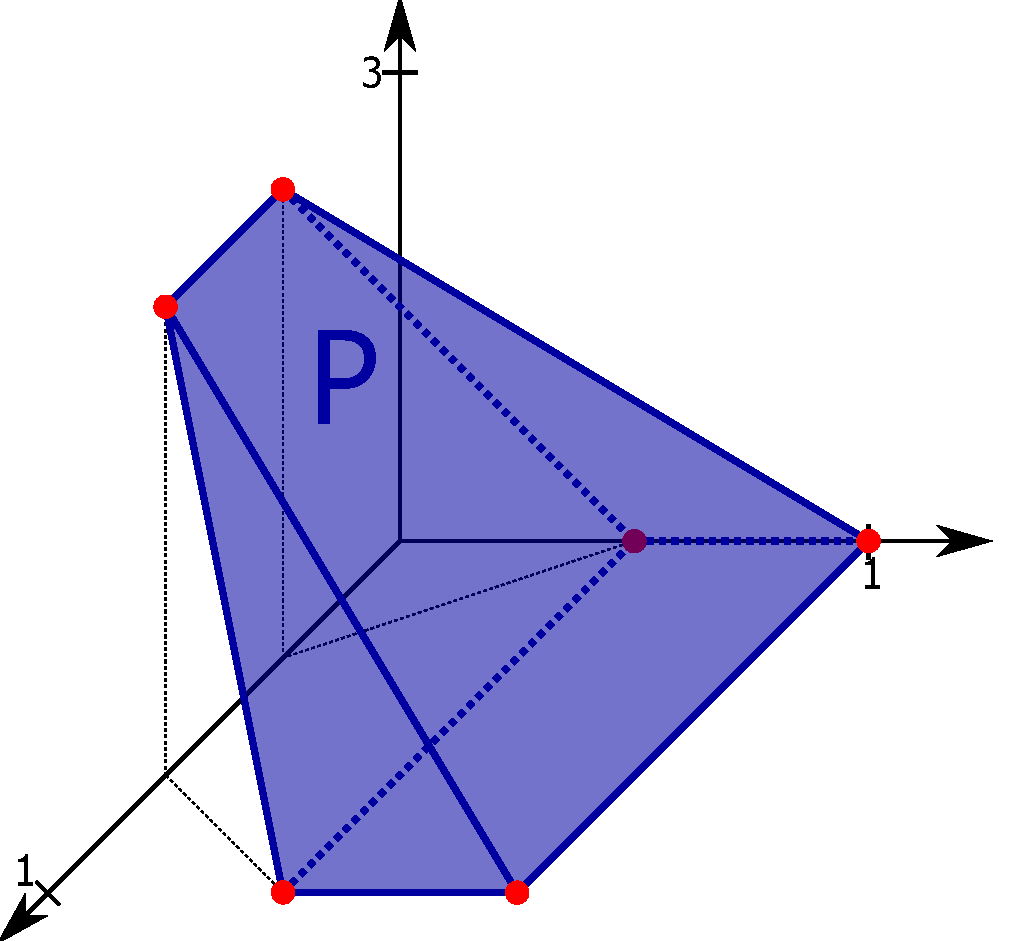
\includegraphics[width=\linewidth]{figs/3dpoly.pdf}
    \end{column}
    \end{columns}
\end{frame}

\begin{frame}
    \frametitle{例}

    \small
    \begin{columns}
    \begin{column}{.3\textwidth}
    $P$: 
    \begin{align*}
        \left\{
        \begin{aligned}
        x_1 + 2x_2 &\leq 6 \\
        2x_1 + x_2 &\leq 6 \\
        x_1 &\geq 0 \\
        x_2 &\geq 0 
        \end{aligned}
        \right.
    \end{align*}
    で定まる$\R^2$の多面体
    \begin{align*}
        \highlight[AlertOrange]{$\tilde A$} =
        \begin{bmatrix}
            1  & 2   \\
            2  & 1   \\
            -1 & 0   \\
            0  & -1
        \end{bmatrix},
        \highlight[UniBlue]{$\tilde b$} = 
        \begin{bmatrix}
            6 \\ 6 \\ 0 \\ 0    
        \end{bmatrix}
    \end{align*}
    \end{column}
    \begin{column}{.7\textwidth}
        \centering
    \begin{tikzpicture}[>=latex,scale=1.3]
        % draw grid
        \draw[gray,very thin] (-.9,-.9) grid (4.5,4.5);
        \node[circle,fill=UniBlue,inner sep=3pt, "{$(0,0)$}" below left] at (0,0) (O) {};
        \node[circle,fill=UniBlue,inner sep=3pt, "{$(3,0)$}" below] at (3,0) (A) {};
        \node[circle,fill=UniBlue,inner sep=3pt, "{$(2,2)$}" above right] at (2,2) (B) {};
        \node[circle,fill=UniBlue,inner sep=3pt, "{$(0,3)$}" above left] at (0,3) (C) {};
        \begin{scope}[on background layer]
            \draw[->,very thick] (-1, 0) -- (4.5,0) node[above] {$x_1$};
            \draw[->,very thick] (0 ,-1) -- (0,4.5) node[left ] {$x_2$};
            \draw[UniBlue, very thick, fill=UniBlue!10] (O.center) -- (A.center) -- (B.center) -- (C.center) -- cycle;
        \end{scope}
        \path (O) -- node[UniBlue,midway,below]{$x_2 \geq 0$} (A);
        \path (A) -- node[UniBlue,midway,above,sloped]{$2x_1 + x_2 \leq 6$} (B);
        \path (B) -- node[UniBlue,midway,above,sloped]{$x_1 + 2x_2 \leq 6$} (C);
        \path (O) -- node[UniBlue,midway,left]{$x_1 \geq 0$} (C);
        \node[UniBlue] at (1,1) {\large $P$};
    \end{tikzpicture}
    \end{column}
    \end{columns}
\end{frame}

%%%%%%%%%%%%%%%%%%%%%%%%%%%%%%%%%%%%%%%%%%%%%%%%%%
\section{整数多面体と完全単模行列}
\againframe<4|handout:0>{outline}
%%%%%%%%%%%%%%%%%%%%%%%%%%%%%%%%%%%%%%%%%%%%%%%%%%
\begin{frame}
    \frametitle{LPを使った組合せ最適化問題の解法?}

    \begin{enumerate}
        \setlength{\itemsep}{1em}
        \item 組合せ最適化問題を\alert{0--1整数計画問題(IP)}として定式化する
        \item IPの0--1制約を落として得られるLPを解く
        \item もし0--1成分のLP最適解が得られたら,それは元のIPの最適解でもあるので,問題が解けた(ラッキー!)
    \end{enumerate}

    \vfill
    これがうまくいくための十分条件は? → \alert{完全単模行列}
\end{frame}

\begin{frame}<1-3>
    \frametitle{例:二部マッチング}

    \small
    \begin{columns}[T]
    \begin{column}{.6\textwidth}
        \begin{block}{重み付き二部マッチング問題}
            \structure{入力} $G=(V; E)$: 二部グラフ,枝重み$w_e$ ($e \in E$) \\
            \structure{出力} $G$の最大重みマッチング$M$
        \end{block}

        \pause
        \begin{block}{\alt<2>{IP}{LP}定式化}
            \setlength{\abovedisplayskip}{0pt}
        \begin{alignat*}{2}
            \text{maximize} & \quad  \sum_{e \in E} w_e x_e \\
            \text{subject to} & \quad \sum_{e \in \delta(i)} x_e \leq 1 & \quad (i \in V) \\
            & \quad \alt<2>{x_e \in \{0,1\}}{} \only<3>{{\color{AlertOrange} x_e \geq 0}} & \quad (e \in E)
        \end{alignat*}
        \end{block}
        \onslide<3->{実は,係数行列の完全単模性により\textbf{常に}0--1のLP最適解をもつ!}
    \end{column}
    \begin{column}{.4\textwidth}
        \centering
        \tikz{
            \graph[nodes={mynodes}, edges={myedges}, grow right=4em]{
            subgraph I_nm [V={1,2,3}, W={4,5}];
            1 -- {4,5};
            2 -- {4,5};
            3 -- {4};
            % matching
            {[edges={mypath}] {1,2} -- {4,5}; }
        };
        }
        \footnotesize
        \begin{alignat*}{3}
            &\text{max}\quad  &&  w^\top x  \\
            &\text{s.t.}\quad  && x_{14} + x_{15}  &&\leq 1 \\
            & && x_{24} + x_{25}  &&\leq 1  \\
            & && x_{34}  &&\leq 1  \\
            & && x_{14} + x_{24} + x_{34} &&\leq 1  \\
            & && x_{15} + x_{25} &&\leq 1  \\
            & && x_{14}, x_{15}, x_{24}, x_{25}, x_{34} &&\in \{0, 1\} 
        \end{alignat*}
    \end{column}
    \end{columns}
\end{frame}


\begin{frame}
    \frametitle{完全単模行列}
    \begin{definition}[完全単模行列]
        $m \times n$行列$A$が\alert{完全単模行列}
        $\defiff$ $A$のすべての小行列式 $\in \{0, \pm 1\}$
    \end{definition}

    \begin{example}
        \[
            \begin{bmatrix}
                1 & 0 \\
                0 & 1
            \end{bmatrix},
            \begin{bmatrix}
                -1 &  1 &  0 & 0  & -1 \\
                1  &  0 &  0 & -1 & 0  \\
                0  & -1 &  1 & 0  & 0  \\
                0  &  0 & -1 & 1  & 1  
            \end{bmatrix} 
        \]
    \end{example}
\end{frame}

\begin{frame}
    \frametitle{例: 二部マッチング}
    
    \small
    \begin{columns}[T]
    \begin{column}{.67\textwidth}
    \begin{lemma}
    二部マッチングのLPの係数行列$A$は完全単模行列.
    \end{lemma}

    \onslide<2->{
    \structure{証明} $k \times k$小行列式$=0,\pm 1$であることを,$k$に関する帰納法で示す.

    $k=1$のときは,$A$の成分は$0,1$なので明らか.

    $k>1$とし,$k \times k$小行列$A'$を考える.
    \footnotesize
   \begin{itemize}
    \item<3-> $A'$にゼロ列が含まれる場合: $\det A' = 0$より成立.
    \item<4-> $A'$に$1$が1つだけ含まれる列がある場合: 余因子展開すれば,$(k-1)\times(k-1)$小行列$A''$を用いて,$\det A' = \pm \det A''$.帰納法の仮定より$\det A'' \in \{0, \pm 1\}$なのでOK.
    \item<5-> $A'$のどの列にも$1$が2つ含まれる場合: 左側の頂点に$+1$,右側の頂点に$-1$をおいた行ベクトル$v$を考えると,$v A' = 0$.よって,$A'$は正則ではないので,$\det A' = 0$. \qed
   \end{itemize} 
    }
    \end{column}
    \begin{column}{.3\textwidth}
        \centering
        \tikz{
            \graph[nodes={mynodes}, edges={myedges}, grow right=4em]{
            subgraph I_nm [V={1,2,3}, W={4,5}];
            1 -- {4,5};
            2 -- {4,5};
            3 -- {4};
        };
        }
        \footnotesize
    \[
        \begin{bNiceMatrix}[first-col=true, first-row=true]
            & x_{14} & x_{15} & x_{24} & x_{25} & x_{34} \\
          1 & 1 & 1 & 0 & 0 & 0 \\
          2 & 0 & 0 & 1 & 1 & 0 \\
          3 & 0 & 0 & 0 & 0 & 1 \\ \hline    
          4 & 1 & 0 & 1 & 0 & 1 \\     
          5 & 0 & 1 & 0 & 1 & 0    
        \end{bNiceMatrix}
    \]
    \end{column}
    \end{columns}

    

\end{frame}


\begin{frame}
    \frametitle{整数多面体}

    \begin{definition}[整数多面体]
       全ての端点が整数ベクトルである多面体を\alert{整数多面体}と呼ぶ.
    \end{definition}
    
    \small
    \begin{columns}[T]
    \begin{column}{.5\textwidth}
        \centering
    \begin{tikzpicture}[>=latex,scale=1.0]
        % draw grid
        \draw[gray,very thin] (-.9,-.9) grid (4.5,3.5);
        \node[circle,fill=UniBlue,inner sep=3pt] at (0,0) (O) {};
        \node[circle,fill=UniBlue,inner sep=3pt] at (3,0) (A) {};
        \node[circle,fill=UniBlue,inner sep=3pt] at (2,2) (B) {};
        \node[circle,fill=UniBlue,inner sep=3pt] at (0,3) (C) {};
        \begin{scope}[on background layer]
            \draw[->,very thick] (-1, 0) -- (4.5,0) node[above] {$x_1$};
            \draw[->,very thick] (0 ,-1) -- (0,3.5) node[left ] {$x_2$};
            \draw[UniBlue, very thick, fill=UniBlue!10] (O.center) -- (A.center) -- (B.center) -- (C.center) -- cycle;
        \end{scope}
    \end{tikzpicture}
    \\  整数多面体
    \end{column}
    \begin{column}{.5\textwidth}
        \centering
    \begin{tikzpicture}[>=latex,scale=1.0]
        % draw grid
        \draw[gray,very thin] (-.9,-.9) grid (4.5,3.5);
        \node[circle,fill=UniBlue,inner sep=3pt] at (0,0) (O) {};
        \node[circle,fill=UniBlue,inner sep=3pt] at (3,0) (A) {};
        \node[circle,fill=AlertOrange,inner sep=3pt] at (2.5,2.5) (B) {};
        \node[circle,fill=UniBlue,inner sep=3pt] at (0,3) (C) {};
        \begin{scope}[on background layer]
            \draw[->,very thick] (-1, 0) -- (4.5,0) node[above] {$x_1$};
            \draw[->,very thick] (0 ,-1) -- (0,3.5) node[left ] {$x_2$};
            \draw[UniBlue, very thick, fill=UniBlue!10] (O.center) -- (A.center) -- (B.center) -- (C.center) -- cycle;
        \end{scope}
    \end{tikzpicture}
    \\ 整数多面体でない多面体
    \end{column}
    \end{columns}
\end{frame}

\begin{frame}
    \frametitle{完全単模行列と整数多面体}

    \small

    \begin{theorem}
        完全単模行列$A$と整数ベクトル$b$が定める多面体
        $
        P = \{ x \in \R^n : Ax \leq b, \, x \geq 0 \} 
        $
    は整数多面体.
    \end{theorem}
    
    \pause
    \structure{証明} \\
    $x$を$P$の端点とする.$x$は,$(\tilde A, \tilde b)$から$n$行を抜き出して得られる正則行列$A'$と部分ベクトル$b'$に対して,線形方程式$A' x = b'$の解$x = (A')^{-1}b'$として得られる.

    \pause
    クラーメルの公式より,
    \[
        (A')^{-1}_{ij} = \frac{\Delta_{j,i} A'}{\det A'} \in \{0,\pm 1\}
    \]
    {\footnotesize ※$\Delta_{j,i} A' = A'$の$(j,i)$余因子}

    $b'$は整数ベクトルなので,$(A')^{-1}b'$も整数ベクトル. \qed

\end{frame}

\begin{frame}
    \frametitle{完全単模行列とLPの整数性}
    
    \begin{columns}[T]
    \begin{column}{.75\textwidth}
    \begin{theorem}[]
        $A$が完全単模行列,$b$が整数ベクトルである主問題(P)を考える.
        もし(P)が最適解をもつならば,(P)に\textbf{整数ベクトル}の最適解が存在する.
    \end{theorem}
    \end{column}
    \begin{column}{.2\textwidth}
        \footnotesize
    \begin{primal}
        \setlength{\abovedisplayskip}{0pt}
        \begin{alignat*}{2}
            \text{max} & \quad  c^\top x \\
            \text{s.t.} & \quad A x \leq b  \\
            & \quad x \geq 0 
        \end{alignat*}
    \end{primal}
    \end{column}
    \end{columns}

    \pause \vfill
    \structure{証明} \\
    前定理より,(P)の実行可能領域$P$は整数多面体である.
    いま,(P)が最適解をもつので,特に$P$の端点である最適解が存在する.
    整数多面体の定義より,これは整数ベクトル. \qed
\end{frame}

\end{document}
